% !TEX program = xelatex
% DeepMIR HW1 report slides. Build: latexmk -xelatex main.tex   (16:9, theme = Moloch, the maintained Metropolis)
\documentclass[aspectratio=169,11pt]{beamer}
\usetheme[progressbar=frametitle]{moloch}        % swap for metropolis / focus / Arguelles to change the look

% ---------- fonts: Fira Sans (ships with TeX Live) + PingFang TC for Chinese ----------
\usepackage{fontspec}
\setsansfont{FiraSans}[Extension=.otf, UprightFont=*-Regular, BoldFont=*-SemiBold, ItalicFont=*-Italic, BoldItalicFont=*-SemiBoldItalic]
\setmonofont{FiraMono}[Extension=.otf, UprightFont=*-Regular, BoldFont=*-Bold, Scale=0.9]
\usepackage{xeCJK}
\setCJKmainfont{PingFangTC-Regular}[BoldFont=PingFangTC-Semibold]
\setCJKsansfont{PingFangTC-Regular}[BoldFont=PingFangTC-Semibold]
\setCJKmonofont{PingFangTC-Regular}

% ---------- packages ----------
\usepackage{booktabs, graphicx, array, multirow}
\usepackage{appendixnumberbeamer}
\graphicspath{{figs/}{../results/}{../eda/}}
\hypersetup{colorlinks=true, urlcolor=orange!80!black, linkcolor=.}

% ---------- helpers ----------
\newcommand{\best}[1]{\textbf{\alert{#1}}}                       % highlight the best number in a table
\newcommand{\fig}[2][0.78\textheight]{\includegraphics[height=#1,keepaspectratio]{#2}}
\newenvironment{tight}{\begin{itemize}\setlength{\itemsep}{1.5pt}\setlength{\parskip}{0pt}\setlength{\topsep}{0pt}}{\end{itemize}}
\newcommand{\src}[1]{\vfill{\scriptsize\color{gray}#1}}          % small source / setting note at the bottom of a slide

\title{Music Era and Release-Market Classification}
\subtitle{DeepMIR 2026 Fall --- Homework 1}
\author{Chi-Jen Peng \quad (R14725022)}
\institute{Code, checkpoints, README: \url{https://github.com/chijenpeng/26-fall-DeepMIR-HW1}}
\date{October 5, 2026}

\begin{document}
\maketitle

% =====================================================================
\section{Experimental Setting}
\begin{frame}{Experimental setting}
  \begin{columns}[T]
    \begin{column}{0.5\textwidth}
      \textbf{Pipeline}
      \begin{itemize}
        \item 30 s clip, 24 kHz mono
        \item frozen encoder $\rightarrow$ mean + std pooling over time
        \item StandardScaler $\rightarrow$ L2 logistic regression
        \item train = fit, validation = model selection, test = prediction file only
      \end{itemize}
    \end{column}
    \begin{column}{0.5\textwidth}
      \textbf{Hardware / software}\\[0.3em]
      {\small
      \begin{tabular}{@{}ll@{}}
        \toprule
        GPU & 2 $\times$ NVIDIA RTX A4500 (20 GB) \\
        CPU / RAM & Intel i9-14900K, 125 GB \\
        OS & Ubuntu 26.04 \\
        Software & PyTorch 2.14, Transformers 4.45,\\ & scikit-learn 1.9 \\
        \bottomrule
      \end{tabular}}
    \end{column}
  \end{columns}
\end{frame}

% =====================================================================
\section{Results}

% ---------------------------------------------------------------- Task 1
\begin{frame}[t]{Task 1: release decade}
  \begin{columns}[T]
    \begin{column}{0.52\textwidth}
      \small
      \textbf{Model}: frozen encoders + logistic regression
      \begin{tight}\footnotesize
        \item Whisper-tiny encoder, \textbf{layer 1}
        \item MERT-v1-330M, \textbf{layers 5, 6, 14}
        \item mean + std pooling over time (6,912-d)
      \end{tight}
      \vspace{0.5em}
      \begin{tabular}{@{}lcc@{}}
        \toprule
        Validation, 132 clips & Top-1 & Top-3 \\ \midrule
        Best model & \best{52.3\%} & \best{86.4\%} \\
        \bottomrule
      \end{tabular}
      \vspace{0.7em}

      \textbf{Errors}
      \begin{tight}\footnotesize
        \item \alert{57\%} of errors land on a \alert{neighboring decade}
        \item Hardest: 2000s (recall .23), absorbed by 2010s and 1990s
        \item Easiest: 1960s and 2010s, which have one neighbor each
      \end{tight}
    \end{column}
    \begin{column}{0.48\textwidth}
      \centering\fig[0.70\textheight]{cm_task1.pdf}\\[-0.2em]
      {\scriptsize\color{gray}Counts. Rows = true decade (22 clips each).}
    \end{column}
  \end{columns}
\end{frame}

\begin{frame}[t]{Why neighbors get confused (1): the low end}
  \begin{columns}[T]
    \begin{column}{0.56\textwidth}
      \small
      \textbf{Hypothesis.} Old masters were cut for vinyl, where deep bass makes the stylus jump, so they should carry less sub-bass.

      \vspace{0.4em}
      \textbf{Analysis.} Long-term average spectrum (Welch) of the 1,026 training clips, split into two bands.

      \vspace{0.5em}
      {\scriptsize\setlength{\tabcolsep}{3.5pt}
      \begin{tabular}{@{}lrrrrrr@{}}
        \toprule
        dB re.\ total & 60s & 70s & 80s & 90s & 00s & 10s \\ \midrule
        20--60 Hz  & \alert{$-21.7$} & $-17.4$ & $-16.0$ & $-14.5$ & $-15.0$ & \alert{$-13.1$} \\
        60--120 Hz & $-8.6$ & $-8.0$ & $-8.1$ & $-7.6$ & $-7.6$ & $-7.1$ \\
        \bottomrule
      \end{tabular}}

      \vspace{0.6em}
      \begin{tight}\footnotesize
        \item Sub-bass rises by \alert{8.6 dB} from the 1960s to the 2010s; the 60--120 Hz band barely moves
        \item From the 1990s on the low end is nearly identical, so it cannot separate 1990s / 2000s / 2010s
      \end{tight}
    \end{column}
    \begin{column}{0.44\textwidth}
      \centering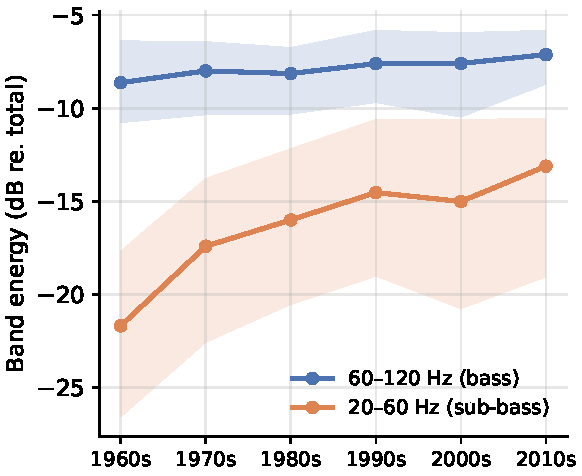
\includegraphics[width=\linewidth]{lowend_trend.pdf}\\[-0.2em]
      {\scriptsize\color{gray}Median and inter-quartile range, training split.}
    \end{column}
  \end{columns}
\end{frame}

\begin{frame}[t]{Why neighbors get confused (2): the loudness war}
  \small
  \textbf{Hypothesis.} From the 2000s, brick-wall limiters push masters louder and flatten the peaks.
  \quad \textbf{Analysis.} Waveform statistics of the training clips.
  \vspace{0.6em}

  \centering
  {\footnotesize
  \begin{tabular}{@{}lrrrrrr@{}}
    \toprule
    Median per decade & 60s & 70s & 80s & 90s & 00s & 10s \\ \midrule
    RMS level (dBFS)                         & $-14.0$ & $-14.6$ & $-14.5$ & $-13.0$ & \alert{$-11.0$} & \alert{$-10.6$} \\
    Crest factor, peak $-$ RMS (dB)          & 13.9 & 14.5 & 14.5 & 13.0 & \alert{11.0} & \alert{10.6} \\
    Dynamic range, loudest 20\% blocks (dB)  & 10.6 & 11.2 & 11.3 & 10.7 & \alert{8.9}  & \alert{8.7} \\
    Longest run pinned at the peak (samples) & 5 & 5 & 6 & 9 & \alert{22} & \alert{26} \\
    Samples within 0.5 dB of the peak (\%)   & 0.02 & 0.01 & 0.02 & 0.06 & \alert{0.42} & \alert{0.50} \\
    \bottomrule
  \end{tabular}}
  \vspace{0.7em}

  \raggedright
  \begin{itemize}
    \item 2000s and 2010s masters are about 3 dB louder with 3 dB less crest, and show the limiter signature: peaks held at the ceiling
    \item The two decades are \alert{almost indistinguishable} on every dynamics measure, matching the 2000s $\leftrightarrow$ 2010s confusion
    \item Production cues only split the data into ``old'' and ``new''; finer distinctions must come from musical content
  \end{itemize}
\end{frame}

% ---------------------------------------------------------------- Task 2
\begin{frame}[t]{Task 2: release market}
  \begin{columns}[T]
    \begin{column}{0.52\textwidth}
      \small
      \textbf{Model}: frozen encoders + logistic regression
      \begin{tight}\footnotesize
        \item Whisper-large-v3 encoder, \textbf{layers 23, 30}
        \item MERT-v1-95M, \textbf{layer 7}
        \item Whisper-small language-ID posteriors
      \end{tight}
      \vspace{0.5em}
      \begin{tabular}{@{}lcc@{}}
        \toprule
        Validation, 102 clips & Top-1 & Top-3 \\ \midrule
        Best model & \best{60.8\%} & \best{90.2\%} \\
        \bottomrule
      \end{tabular}
      \vspace{0.7em}

      \textbf{Errors}
      \begin{tight}\footnotesize
        \item \alert{75\%} of errors are among \alert{US, UK, Germany, Italy}
        \item Largest confused pair: US $\leftrightarrow$ UK (9 clips)
        \item Brazil (.88) and Spain (.82) are rarely missed
        \item Cause: English-language releases dominate Germany (83\%) and Italy (55\%)
      \end{tight}
    \end{column}
    \begin{column}{0.48\textwidth}
      \centering\fig[0.70\textheight]{cm_task2.pdf}\\[-0.2em]
      {\scriptsize\color{gray}Counts. Rows = true market (17 clips each).}
    \end{column}
  \end{columns}
\end{frame}

% =====================================================================
\section{Optional Experiments}
\begin{frame}{Input length: 5 / 10 / 15 / 30 s}
  % TODO
\end{frame}

% =====================================================================
\section{Ablation}
\begin{frame}{Frozen features vs.\ fine-tuning}
  % TODO
\end{frame}

% =====================================================================
\section{Audio Language Model}
\begin{frame}{Qwen2-Audio, zero-shot}
  % TODO
\end{frame}

% =====================================================================
\section{Disclosure}
\begin{frame}{Use of AI assistance}
  % TODO: statement from report_outline.md section 5
\end{frame}

% =====================================================================
\section{References}
\begin{frame}[allowframebreaks]{References}
  \footnotesize
  % TODO: list from report_outline.md section 6
\end{frame}

\end{document}
